\PassOptionsToPackage{unicode=true}{hyperref} % options for packages loaded elsewhere
\PassOptionsToPackage{hyphens}{url}
%
\documentclass[
  ignorenonframetext,
]{beamer}
\usepackage{pgfpages}
\setbeamertemplate{caption}[numbered]
\setbeamertemplate{caption label separator}{: }
\setbeamercolor{caption name}{fg=normal text.fg}
\beamertemplatenavigationsymbolsempty
% Prevent slide breaks in the middle of a paragraph:
\widowpenalties 1 10000
\raggedbottom
\setbeamertemplate{part page}{
  \centering
  \begin{beamercolorbox}[sep=16pt,center]{part title}
    \usebeamerfont{part title}\insertpart\par
  \end{beamercolorbox}
}
\setbeamertemplate{section page}{
  \centering
  \begin{beamercolorbox}[sep=12pt,center]{part title}
    \usebeamerfont{section title}\insertsection\par
  \end{beamercolorbox}
}
\setbeamertemplate{subsection page}{
  \centering
  \begin{beamercolorbox}[sep=8pt,center]{part title}
    \usebeamerfont{subsection title}\insertsubsection\par
  \end{beamercolorbox}
}
\AtBeginPart{
  \frame{\partpage}
}
\AtBeginSection{
  \ifbibliography
  \else
    \frame{\sectionpage}
  \fi
}
\AtBeginSubsection{
  \frame{\subsectionpage}
}
\usepackage{lmodern}
\usepackage{amssymb,amsmath}
\usepackage{ifxetex,ifluatex}
\ifnum 0\ifxetex 1\fi\ifluatex 1\fi=0 % if pdftex
  \usepackage[T1]{fontenc}
  \usepackage[utf8]{inputenc}
  \usepackage{textcomp} % provides euro and other symbols
\else % if luatex or xelatex
  \usepackage{unicode-math}
  \defaultfontfeatures{Scale=MatchLowercase}
  \defaultfontfeatures[\rmfamily]{Ligatures=TeX,Scale=1}
\fi
\usetheme[]{CambridgeUS}
\usecolortheme{beaver}
\usefonttheme{structurebold}
% use upquote if available, for straight quotes in verbatim environments
\IfFileExists{upquote.sty}{\usepackage{upquote}}{}
\IfFileExists{microtype.sty}{% use microtype if available
  \usepackage[]{microtype}
  \UseMicrotypeSet[protrusion]{basicmath} % disable protrusion for tt fonts
}{}
\makeatletter
\@ifundefined{KOMAClassName}{% if non-KOMA class
  \IfFileExists{parskip.sty}{%
    \usepackage{parskip}
  }{% else
    \setlength{\parindent}{0pt}
    \setlength{\parskip}{6pt plus 2pt minus 1pt}}
}{% if KOMA class
  \KOMAoptions{parskip=half}}
\makeatother
\usepackage{xcolor}
\IfFileExists{xurl.sty}{\usepackage{xurl}}{} % add URL line breaks if available
\IfFileExists{bookmark.sty}{\usepackage{bookmark}}{\usepackage{hyperref}}
\hypersetup{
  pdftitle={Lineare Regression},
  pdfauthor={Jan-Philipp Kolb},
  pdfborder={0 0 0},
  breaklinks=true}
\urlstyle{same}  % don't use monospace font for urls
\newif\ifbibliography
\usepackage{color}
\usepackage{fancyvrb}
\newcommand{\VerbBar}{|}
\newcommand{\VERB}{\Verb[commandchars=\\\{\}]}
\DefineVerbatimEnvironment{Highlighting}{Verbatim}{commandchars=\\\{\}}
% Add ',fontsize=\small' for more characters per line
\usepackage{framed}
\definecolor{shadecolor}{RGB}{42,33,28}
\newenvironment{Shaded}{\begin{snugshade}}{\end{snugshade}}
\newcommand{\AlertTok}[1]{\textcolor[rgb]{1.00,1.00,0.00}{#1}}
\newcommand{\AnnotationTok}[1]{\textcolor[rgb]{0.00,0.40,1.00}{\textbf{\textit{#1}}}}
\newcommand{\AttributeTok}[1]{\textcolor[rgb]{0.74,0.68,0.62}{#1}}
\newcommand{\BaseNTok}[1]{\textcolor[rgb]{0.27,0.67,0.26}{#1}}
\newcommand{\BuiltInTok}[1]{\textcolor[rgb]{0.74,0.68,0.62}{#1}}
\newcommand{\CharTok}[1]{\textcolor[rgb]{0.02,0.61,0.04}{#1}}
\newcommand{\CommentTok}[1]{\textcolor[rgb]{0.00,0.40,1.00}{\textbf{\textit{#1}}}}
\newcommand{\CommentVarTok}[1]{\textcolor[rgb]{0.74,0.68,0.62}{#1}}
\newcommand{\ConstantTok}[1]{\textcolor[rgb]{0.74,0.68,0.62}{#1}}
\newcommand{\ControlFlowTok}[1]{\textcolor[rgb]{0.26,0.66,0.93}{\textbf{#1}}}
\newcommand{\DataTypeTok}[1]{\textcolor[rgb]{0.74,0.68,0.62}{\underline{#1}}}
\newcommand{\DecValTok}[1]{\textcolor[rgb]{0.27,0.67,0.26}{#1}}
\newcommand{\DocumentationTok}[1]{\textcolor[rgb]{0.00,0.40,1.00}{\textit{#1}}}
\newcommand{\ErrorTok}[1]{\textcolor[rgb]{1.00,1.00,0.00}{\textbf{#1}}}
\newcommand{\ExtensionTok}[1]{\textcolor[rgb]{0.74,0.68,0.62}{#1}}
\newcommand{\FloatTok}[1]{\textcolor[rgb]{0.27,0.67,0.26}{#1}}
\newcommand{\FunctionTok}[1]{\textcolor[rgb]{1.00,0.58,0.35}{\textbf{#1}}}
\newcommand{\ImportTok}[1]{\textcolor[rgb]{0.74,0.68,0.62}{#1}}
\newcommand{\InformationTok}[1]{\textcolor[rgb]{0.00,0.40,1.00}{\textbf{\textit{#1}}}}
\newcommand{\KeywordTok}[1]{\textcolor[rgb]{0.26,0.66,0.93}{\textbf{#1}}}
\newcommand{\NormalTok}[1]{\textcolor[rgb]{0.74,0.68,0.62}{#1}}
\newcommand{\OperatorTok}[1]{\textcolor[rgb]{0.74,0.68,0.62}{#1}}
\newcommand{\OtherTok}[1]{\textcolor[rgb]{0.74,0.68,0.62}{#1}}
\newcommand{\PreprocessorTok}[1]{\textcolor[rgb]{0.74,0.68,0.62}{\textbf{#1}}}
\newcommand{\RegionMarkerTok}[1]{\textcolor[rgb]{0.74,0.68,0.62}{#1}}
\newcommand{\SpecialCharTok}[1]{\textcolor[rgb]{0.02,0.61,0.04}{#1}}
\newcommand{\SpecialStringTok}[1]{\textcolor[rgb]{0.02,0.61,0.04}{#1}}
\newcommand{\StringTok}[1]{\textcolor[rgb]{0.02,0.61,0.04}{#1}}
\newcommand{\VariableTok}[1]{\textcolor[rgb]{0.74,0.68,0.62}{#1}}
\newcommand{\VerbatimStringTok}[1]{\textcolor[rgb]{0.02,0.61,0.04}{#1}}
\newcommand{\WarningTok}[1]{\textcolor[rgb]{1.00,1.00,0.00}{\textbf{#1}}}
\usepackage{longtable,booktabs}
\usepackage{caption}
% These lines are needed to make table captions work with longtable:
\makeatletter
\def\fnum@table{\tablename~\thetable}
\makeatother
\usepackage{graphicx,grffile}
\makeatletter
\def\maxwidth{\ifdim\Gin@nat@width>\linewidth\linewidth\else\Gin@nat@width\fi}
\def\maxheight{\ifdim\Gin@nat@height>\textheight\textheight\else\Gin@nat@height\fi}
\makeatother
% Scale images if necessary, so that they will not overflow the page
% margins by default, and it is still possible to overwrite the defaults
% using explicit options in \includegraphics[width, height, ...]{}
\setkeys{Gin}{width=\maxwidth,height=\maxheight,keepaspectratio}
\setlength{\emergencystretch}{3em}  % prevent overfull lines
\providecommand{\tightlist}{%
  \setlength{\itemsep}{0pt}\setlength{\parskip}{0pt}}
\setcounter{secnumdepth}{-2}

% set default figure placement to htbp
\makeatletter
\def\fps@figure{htbp}
\makeatother


\title{Lineare Regression}
\author{Jan-Philipp Kolb}
\date{06 Mai, 2019}

\begin{document}
\frame{\titlepage}

\begin{frame}{Die lineare Regression}
\protect\hypertarget{die-lineare-regression}{}

Maindonald -
\href{https://cran.r-project.org/doc/contrib/usingR.pdf}{DataAnalysis}

\begin{itemize}
\tightlist
\item
  Einführung in R
\item
  Datenanalyse
\item
  Statistische Modelle
\item
  Inferenzkonzepte
\item
  Regression mit einem Prädiktor
\item
  Multiple lineare Regression
\item
  Ausweitung des linearen Modells
\item
  \ldots{}
\end{itemize}

\end{frame}

\begin{frame}[fragile]{Lineare Regression in R - Beispieldatensatz}
\protect\hypertarget{lineare-regression-in-r---beispieldatensatz}{}

John H. Maindonald and W. John Braun

DAAG -
\href{http://cran.ms.unimelb.edu.au/web/packages/DAAG/DAAG.pdf}{Data
Analysis and Graphics Data and Functions}

\begin{Shaded}
\begin{Highlighting}[]
\KeywordTok{install.packages}\NormalTok{(}\StringTok{"DAAG"}\NormalTok{)}
\end{Highlighting}
\end{Shaded}

\begin{Shaded}
\begin{Highlighting}[]
\KeywordTok{library}\NormalTok{(}\StringTok{"DAAG"}\NormalTok{)}
\KeywordTok{data}\NormalTok{(roller)}
\end{Highlighting}
\end{Shaded}

Hilfe für den \texttt{roller} Datensatz:

\begin{Shaded}
\begin{Highlighting}[]
\NormalTok{?roller}
\end{Highlighting}
\end{Shaded}

\begin{Shaded}
\begin{Highlighting}[]
\NormalTok{roller}
\end{Highlighting}
\end{Shaded}

\end{frame}

\begin{frame}{Variablen des \texttt{mtcars} Datensatzes}
\protect\hypertarget{variablen-des-mtcars-datensatzes}{}

\begin{itemize}
\tightlist
\item
  mpg - Miles/(US) gallon
\item
  cyl - Number of cylinders
\item
  disp - Displacement (cu.in.)
\item
  hp - Gross horsepower
\item
  drat - Rear axle ratio
\item
  wt - Weight (1000 lbs)
\item
  qsec - 1/4 mile time
\item
  vs - Engine (0 = V-shaped, 1 = straight)
\item
  am - Transmission (0 = automatic, 1 = manual)
\item
  gear - Number of forward gears
\item
  carb - Number of carburetors
\end{itemize}

\end{frame}

\begin{frame}{Datensatz \texttt{mtcars}}
\protect\hypertarget{datensatz-mtcars}{}

\begin{longtable}[]{@{}lrrrrrrrrrrr@{}}
\toprule
& mpg & cyl & disp & hp & drat & wt & qsec & vs & am & gear &
carb\tabularnewline
\midrule
\endhead
Mazda RX4 & 21.0 & 6 & 160.0 & 110 & 3.90 & 2.620 & 16.46 & 0 & 1 & 4 &
4\tabularnewline
Mazda RX4 Wag & 21.0 & 6 & 160.0 & 110 & 3.90 & 2.875 & 17.02 & 0 & 1 &
4 & 4\tabularnewline
Datsun 710 & 22.8 & 4 & 108.0 & 93 & 3.85 & 2.320 & 18.61 & 1 & 1 & 4 &
1\tabularnewline
Hornet 4 Drive & 21.4 & 6 & 258.0 & 110 & 3.08 & 3.215 & 19.44 & 1 & 0 &
3 & 1\tabularnewline
Hornet Sportabout & 18.7 & 8 & 360.0 & 175 & 3.15 & 3.440 & 17.02 & 0 &
0 & 3 & 2\tabularnewline
Valiant & 18.1 & 6 & 225.0 & 105 & 2.76 & 3.460 & 20.22 & 1 & 0 & 3 &
1\tabularnewline
Duster 360 & 14.3 & 8 & 360.0 & 245 & 3.21 & 3.570 & 15.84 & 0 & 0 & 3 &
4\tabularnewline
Merc 240D & 24.4 & 4 & 146.7 & 62 & 3.69 & 3.190 & 20.00 & 1 & 0 & 4 &
2\tabularnewline
Merc 230 & 22.8 & 4 & 140.8 & 95 & 3.92 & 3.150 & 22.90 & 1 & 0 & 4 &
2\tabularnewline
Merc 280 & 19.2 & 6 & 167.6 & 123 & 3.92 & 3.440 & 18.30 & 1 & 0 & 4 &
4\tabularnewline
Merc 280C & 17.8 & 6 & 167.6 & 123 & 3.92 & 3.440 & 18.90 & 1 & 0 & 4 &
4\tabularnewline
Merc 450SE & 16.4 & 8 & 275.8 & 180 & 3.07 & 4.070 & 17.40 & 0 & 0 & 3 &
3\tabularnewline
Merc 450SL & 17.3 & 8 & 275.8 & 180 & 3.07 & 3.730 & 17.60 & 0 & 0 & 3 &
3\tabularnewline
Merc 450SLC & 15.2 & 8 & 275.8 & 180 & 3.07 & 3.780 & 18.00 & 0 & 0 & 3
& 3\tabularnewline
Cadillac Fleetwood & 10.4 & 8 & 472.0 & 205 & 2.93 & 5.250 & 17.98 & 0 &
0 & 3 & 4\tabularnewline
Lincoln Continental & 10.4 & 8 & 460.0 & 215 & 3.00 & 5.424 & 17.82 & 0
& 0 & 3 & 4\tabularnewline
Chrysler Imperial & 14.7 & 8 & 440.0 & 230 & 3.23 & 5.345 & 17.42 & 0 &
0 & 3 & 4\tabularnewline
Fiat 128 & 32.4 & 4 & 78.7 & 66 & 4.08 & 2.200 & 19.47 & 1 & 1 & 4 &
1\tabularnewline
Honda Civic & 30.4 & 4 & 75.7 & 52 & 4.93 & 1.615 & 18.52 & 1 & 1 & 4 &
2\tabularnewline
Toyota Corolla & 33.9 & 4 & 71.1 & 65 & 4.22 & 1.835 & 19.90 & 1 & 1 & 4
& 1\tabularnewline
Toyota Corona & 21.5 & 4 & 120.1 & 97 & 3.70 & 2.465 & 20.01 & 1 & 0 & 3
& 1\tabularnewline
Dodge Challenger & 15.5 & 8 & 318.0 & 150 & 2.76 & 3.520 & 16.87 & 0 & 0
& 3 & 2\tabularnewline
AMC Javelin & 15.2 & 8 & 304.0 & 150 & 3.15 & 3.435 & 17.30 & 0 & 0 & 3
& 2\tabularnewline
Camaro Z28 & 13.3 & 8 & 350.0 & 245 & 3.73 & 3.840 & 15.41 & 0 & 0 & 3 &
4\tabularnewline
Pontiac Firebird & 19.2 & 8 & 400.0 & 175 & 3.08 & 3.845 & 17.05 & 0 & 0
& 3 & 2\tabularnewline
Fiat X1-9 & 27.3 & 4 & 79.0 & 66 & 4.08 & 1.935 & 18.90 & 1 & 1 & 4 &
1\tabularnewline
Porsche 914-2 & 26.0 & 4 & 120.3 & 91 & 4.43 & 2.140 & 16.70 & 0 & 1 & 5
& 2\tabularnewline
Lotus Europa & 30.4 & 4 & 95.1 & 113 & 3.77 & 1.513 & 16.90 & 1 & 1 & 5
& 2\tabularnewline
Ford Pantera L & 15.8 & 8 & 351.0 & 264 & 4.22 & 3.170 & 14.50 & 0 & 1 &
5 & 4\tabularnewline
Ferrari Dino & 19.7 & 6 & 145.0 & 175 & 3.62 & 2.770 & 15.50 & 0 & 1 & 5
& 6\tabularnewline
Maserati Bora & 15.0 & 8 & 301.0 & 335 & 3.54 & 3.570 & 14.60 & 0 & 1 &
5 & 8\tabularnewline
Volvo 142E & 21.4 & 4 & 121.0 & 109 & 4.11 & 2.780 & 18.60 & 1 & 1 & 4 &
2\tabularnewline
\bottomrule
\end{longtable}

\end{frame}

\begin{frame}[fragile]{Verteilungen für zwei Variablen von
\texttt{mtcars}}
\protect\hypertarget{verteilungen-fur-zwei-variablen-von-mtcars}{}

\begin{Shaded}
\begin{Highlighting}[]
\KeywordTok{par}\NormalTok{(}\DataTypeTok{mfrow=}\KeywordTok{c}\NormalTok{(}\DecValTok{1}\NormalTok{,}\DecValTok{2}\NormalTok{))}
\KeywordTok{plot}\NormalTok{(}\KeywordTok{density}\NormalTok{(mtcars}\OperatorTok{$}\NormalTok{wt)); }\KeywordTok{plot}\NormalTok{(}\KeywordTok{density}\NormalTok{(mtcars}\OperatorTok{$}\NormalTok{mpg))}
\end{Highlighting}
\end{Shaded}

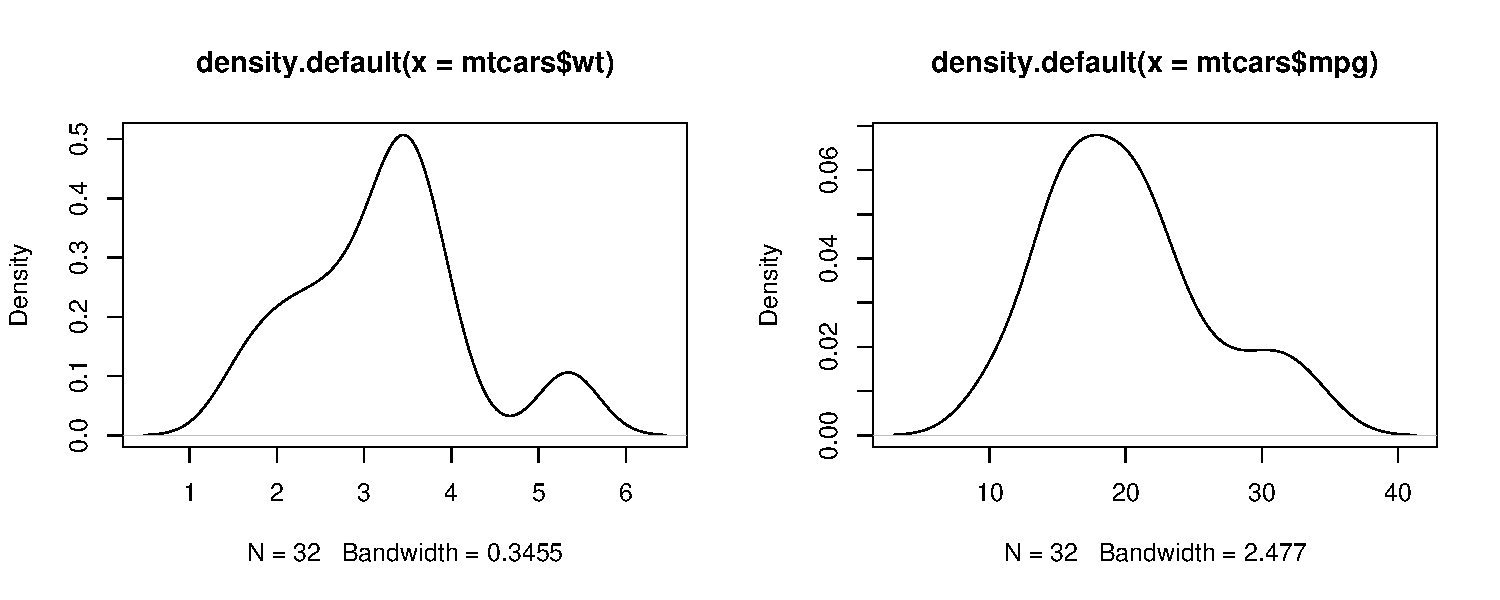
\includegraphics{LineareRegression_files/figure-beamer/unnamed-chunk-7-1.pdf}

\end{frame}

\begin{frame}[fragile]{Ein einfaches Regressionsmodell}
\protect\hypertarget{ein-einfaches-regressionsmodell}{}

\begin{block}{Abhängige Variable - Meilen pro Gallone (\texttt{mpg})}

\end{block}

\begin{block}{Unabhängige Variable - Gewicht (\texttt{wt})}

\begin{Shaded}
\begin{Highlighting}[]
\NormalTok{m1 <-}\StringTok{ }\KeywordTok{lm}\NormalTok{(mpg }\OperatorTok{~}\StringTok{ }\NormalTok{wt,}\DataTypeTok{data=}\NormalTok{mtcars)}
\NormalTok{m1}
\end{Highlighting}
\end{Shaded}

\begin{verbatim}
## 
## Call:
## lm(formula = mpg ~ wt, data = mtcars)
## 
## Coefficients:
## (Intercept)           wt  
##      37.285       -5.344
\end{verbatim}

\end{block}

\end{frame}

\begin{frame}[fragile]{Die Modellformel}
\protect\hypertarget{die-modellformel}{}

\begin{block}{Modell ohne Achsenabschnitt}

\begin{Shaded}
\begin{Highlighting}[]
\NormalTok{m2 <-}\StringTok{ }\KeywordTok{lm}\NormalTok{(mpg }\OperatorTok{~}\StringTok{ }\OperatorTok{-}\StringTok{ }\DecValTok{1} \OperatorTok{+}\StringTok{ }\NormalTok{wt,}\DataTypeTok{data=}\NormalTok{mtcars)}
\KeywordTok{summary}\NormalTok{(m2)}\OperatorTok{$}\NormalTok{coefficients}
\end{Highlighting}
\end{Shaded}

\begin{verbatim}
##    Estimate Std. Error  t value    Pr(>|t|)
## wt 5.291624  0.5931801 8.920771 4.55314e-10
\end{verbatim}

\end{block}

\begin{block}{Weitere Variablen hinzufügen}

\begin{Shaded}
\begin{Highlighting}[]
\NormalTok{m3 <-}\StringTok{ }\KeywordTok{lm}\NormalTok{(mpg }\OperatorTok{~}\StringTok{ }\NormalTok{wt }\OperatorTok{+}\StringTok{ }\NormalTok{cyl,}\DataTypeTok{data=}\NormalTok{mtcars)}
\KeywordTok{summary}\NormalTok{(m3)}\OperatorTok{$}\NormalTok{coefficients}
\end{Highlighting}
\end{Shaded}

\begin{verbatim}
##              Estimate Std. Error   t value     Pr(>|t|)
## (Intercept) 39.686261  1.7149840 23.140893 3.043182e-20
## wt          -3.190972  0.7569065 -4.215808 2.220200e-04
## cyl         -1.507795  0.4146883 -3.635972 1.064282e-03
\end{verbatim}

\end{block}

\end{frame}

\begin{frame}[fragile]{Summary des Modells}
\protect\hypertarget{summary-des-modells}{}

\begin{Shaded}
\begin{Highlighting}[]
\KeywordTok{summary}\NormalTok{(m3)}
\end{Highlighting}
\end{Shaded}

\begin{verbatim}
## 
## Call:
## lm(formula = mpg ~ wt + cyl, data = mtcars)
## 
## Residuals:
##     Min      1Q  Median      3Q     Max 
## -4.2893 -1.5512 -0.4684  1.5743  6.1004 
## 
## Coefficients:
##             Estimate Std. Error t value Pr(>|t|)    
## (Intercept)  39.6863     1.7150  23.141  < 2e-16 ***
## wt           -3.1910     0.7569  -4.216 0.000222 ***
## cyl          -1.5078     0.4147  -3.636 0.001064 ** 
## ---
## Signif. codes:  0 '***' 0.001 '**' 0.01 '*' 0.05 '.' 0.1 ' ' 1
## 
## Residual standard error: 2.568 on 29 degrees of freedom
## Multiple R-squared:  0.8302, Adjusted R-squared:  0.8185 
## F-statistic: 70.91 on 2 and 29 DF,  p-value: 6.809e-12
\end{verbatim}

\end{frame}

\begin{frame}[fragile]{R arbeitet mit Objekten}
\protect\hypertarget{r-arbeitet-mit-objekten}{}

\begin{itemize}
\tightlist
\item
  \texttt{m3} ist nun ein spezielles Regressions-Objekt
\item
  Auf dieses Objekt können nun verschiedene Funktionen angewendet werden
\end{itemize}

\begin{Shaded}
\begin{Highlighting}[]
\KeywordTok{predict}\NormalTok{(m3) }\CommentTok{# Vorhersage}
\end{Highlighting}
\end{Shaded}

\begin{verbatim}
##           Mazda RX4       Mazda RX4 Wag          Datsun 710 
##            22.27914            21.46545            26.25203 
##      Hornet 4 Drive   Hornet Sportabout             Valiant 
##            20.38052            16.64696            19.59873 
##          Duster 360           Merc 240D            Merc 230 
##            16.23213            23.47588            23.60352 
##            Merc 280           Merc 280C          Merc 450SE 
##            19.66255            19.66255            14.63665 
##          Merc 450SL         Merc 450SLC  Cadillac Fleetwood 
##            15.72158            15.56203            10.87130 
## Lincoln Continental   Chrysler Imperial            Fiat 128 
##            10.31607            10.56816            26.63494 
##         Honda Civic      Toyota Corolla       Toyota Corona 
##            28.50166            27.79965            25.78934 
##    Dodge Challenger         AMC Javelin          Camaro Z28 
##            16.39168            16.66291            15.37057 
##    Pontiac Firebird           Fiat X1-9       Porsche 914-2 
##            15.35461            27.48055            26.82640 
##        Lotus Europa      Ford Pantera L        Ferrari Dino 
##            28.82714            17.50852            21.80050 
##       Maserati Bora          Volvo 142E 
##            16.23213            24.78418
\end{verbatim}

\begin{Shaded}
\begin{Highlighting}[]
\KeywordTok{resid}\NormalTok{(m3) }\CommentTok{# Residuen}
\end{Highlighting}
\end{Shaded}

\begin{verbatim}
##           Mazda RX4       Mazda RX4 Wag          Datsun 710 
##         -1.27914467         -0.46544677         -3.45202624 
##      Hornet 4 Drive   Hornet Sportabout             Valiant 
##          1.01948376          2.05304242         -1.49872807 
##          Duster 360           Merc 240D            Merc 230 
##         -1.93213120          0.92411952         -0.80351937 
##            Merc 280           Merc 280C          Merc 450SE 
##         -0.46254751         -1.86254751          1.76335487 
##          Merc 450SL         Merc 450SLC  Cadillac Fleetwood 
##          1.57842434         -0.36202705         -0.47129800 
## Lincoln Continental   Chrysler Imperial            Fiat 128 
##          0.08393115          4.13184435          5.76505710 
##         Honda Civic      Toyota Corolla       Toyota Corona 
##          1.89833840          6.10035227         -4.28933528 
##    Dodge Challenger         AMC Javelin          Camaro Z28 
##         -0.89167980         -1.46291244         -2.07056872 
##    Pontiac Firebird           Fiat X1-9       Porsche 914-2 
##          3.84538614         -0.18055052         -0.82640123 
##        Lotus Europa      Ford Pantera L        Ferrari Dino 
##          1.57285924         -1.70852005         -2.10049885 
##       Maserati Bora          Volvo 142E 
##         -1.23213120         -3.38417906
\end{verbatim}

\end{frame}

\begin{frame}[fragile]{Residuenplot}
\protect\hypertarget{residuenplot}{}

\begin{itemize}
\tightlist
\item
  Sind Annahmen des linearen Regressionsmodells verletzt?
\item
  Dies ist der Fall, wenn ein Muster abweichend von einer Linie zu
  erkennen ist.
\item
  Hier ist der Datensatz sehr klein
\end{itemize}

\begin{Shaded}
\begin{Highlighting}[]
\KeywordTok{plot}\NormalTok{(m3,}\DecValTok{1}\NormalTok{)}
\end{Highlighting}
\end{Shaded}

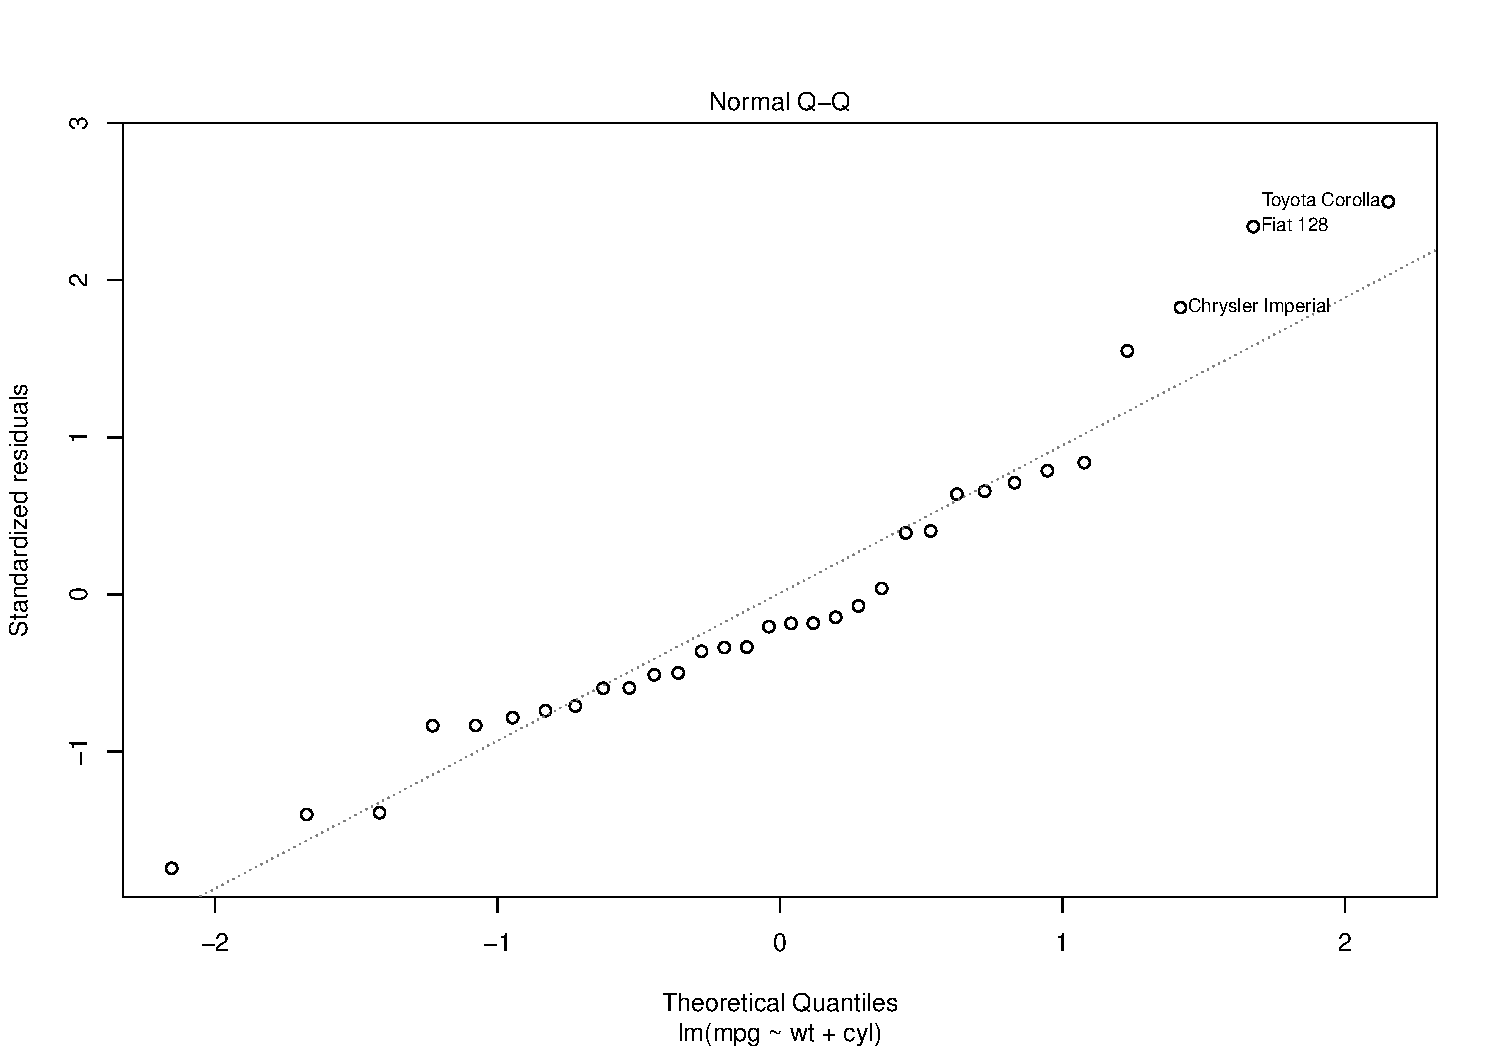
\includegraphics{LineareRegression_files/figure-beamer/unnamed-chunk-13-1.pdf}

\end{frame}

\begin{frame}[fragile]{Residuenplot}
\protect\hypertarget{residuenplot-1}{}

\begin{Shaded}
\begin{Highlighting}[]
\KeywordTok{plot}\NormalTok{(m3,}\DecValTok{2}\NormalTok{)}
\end{Highlighting}
\end{Shaded}


\includegraphics{LineareRegression_files/figure-beamer/unnamed-chunk-14-1.pdf}

\begin{itemize}
\tightlist
\item
  Wenn die Residuen normalverteilt sind sollten sie auf einer Linie
  liegen.
\end{itemize}

\end{frame}

\begin{frame}[fragile]{\href{https://cran.r-project.org/web/packages/Formula/vignettes/Formula.pdf}{Weitere
Möglichkeiten die Formel zu spezifizieren}}
\protect\hypertarget{weitere-moglichkeiten-die-formel-zu-spezifizieren}{}

\begin{block}{Interaktionseffekt}

\begin{Shaded}
\begin{Highlighting}[]
\CommentTok{# effect of cyl and interaction effect:}
\NormalTok{m3a<-}\KeywordTok{lm}\NormalTok{(mpg}\OperatorTok{~}\NormalTok{wt}\OperatorTok{*}\NormalTok{cyl,}\DataTypeTok{data=}\NormalTok{mtcars) }

\CommentTok{# only interaction effect:}
\NormalTok{m3b<-}\KeywordTok{lm}\NormalTok{(mpg}\OperatorTok{~}\NormalTok{wt}\OperatorTok{:}\NormalTok{cyl,}\DataTypeTok{data=}\NormalTok{mtcars) }
\end{Highlighting}
\end{Shaded}

\end{block}

\begin{block}{Den Logarithmus nehmen}

\begin{Shaded}
\begin{Highlighting}[]
\NormalTok{m3d<-}\KeywordTok{lm}\NormalTok{(mpg}\OperatorTok{~}\KeywordTok{log}\NormalTok{(wt),}\DataTypeTok{data=}\NormalTok{mtcars) }
\end{Highlighting}
\end{Shaded}

\end{block}

\end{frame}

\begin{frame}[fragile]{Ein Modell mit Interaktionseffekt}
\protect\hypertarget{ein-modell-mit-interaktionseffekt}{}

-\texttt{disp} - Hubraum

\begin{Shaded}
\begin{Highlighting}[]
\NormalTok{m3d<-}\KeywordTok{lm}\NormalTok{(mpg}\OperatorTok{~}\NormalTok{wt}\OperatorTok{*}\NormalTok{disp,}\DataTypeTok{data=}\NormalTok{mtcars) }
\NormalTok{m3dsum <-}\StringTok{ }\KeywordTok{summary}\NormalTok{(m3d)}
\NormalTok{m3dsum}\OperatorTok{$}\NormalTok{coefficients}
\end{Highlighting}
\end{Shaded}

\begin{verbatim}
##                Estimate  Std. Error   t value     Pr(>|t|)
## (Intercept) 44.08199770 3.123062627 14.114990 2.955567e-14
## wt          -6.49567966 1.313382622 -4.945763 3.216705e-05
## disp        -0.05635816 0.013238696 -4.257078 2.101721e-04
## wt:disp      0.01170542 0.003255102  3.596022 1.226988e-03
\end{verbatim}

\end{frame}

\begin{frame}[fragile]{\href{https://cran.r-project.org/web/packages/jtools/vignettes/interactions.html}{Interaktionen
untersuchen}}
\protect\hypertarget{interaktionen-untersuchen}{}

\begin{Shaded}
\begin{Highlighting}[]
\KeywordTok{install.packages}\NormalTok{(}\StringTok{"jtools"}\NormalTok{)}
\end{Highlighting}
\end{Shaded}

\begin{Shaded}
\begin{Highlighting}[]
\KeywordTok{library}\NormalTok{(jtools)}
\KeywordTok{interact_plot}\NormalTok{(m3d, }\DataTypeTok{pred =} \StringTok{"wt"}\NormalTok{, }\DataTypeTok{modx =} \StringTok{"disp"}\NormalTok{)}
\end{Highlighting}
\end{Shaded}

\begin{itemize}
\tightlist
\item
  Mit einem kontinuierlichen Moderator (in unserem Fall \texttt{Disp})
  erhält man drei Zeilen - 1 Standardabweichung über und unter dem
  Mittelwert und der Mittelwert selbst.
\end{itemize}

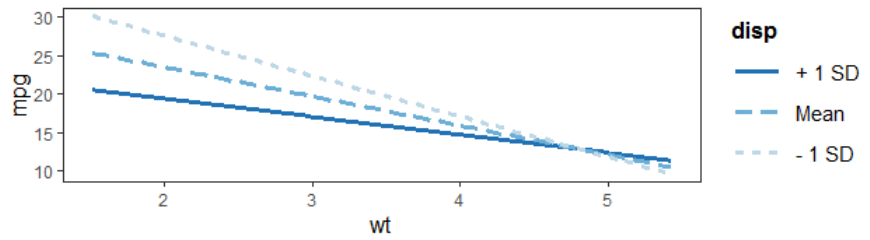
\includegraphics{figure/mtcars_model_interact.PNG}

\end{frame}

\begin{frame}[fragile]{Das Paket \texttt{interplot}}
\protect\hypertarget{das-paket-interplot}{}

\begin{Shaded}
\begin{Highlighting}[]
\KeywordTok{library}\NormalTok{(interplot)}
\end{Highlighting}
\end{Shaded}

\begin{itemize}
\tightlist
\item
  Effekt wird auf die y-Achse geplottet - \texttt{wt} auf der x-Achse
\end{itemize}

\begin{Shaded}
\begin{Highlighting}[]
\KeywordTok{interplot}\NormalTok{(}\DataTypeTok{m =}\NormalTok{ m3a, }\DataTypeTok{var1 =} \StringTok{"wt"}\NormalTok{, }\DataTypeTok{var2 =} \StringTok{"disp"}\NormalTok{, }\DataTypeTok{hist =} \OtherTok{TRUE}\NormalTok{)  }
\end{Highlighting}
\end{Shaded}

\includegraphics{figure/interplot_wt_disp.PNG}

\begin{itemize}
\tightlist
\item
  Eine detailliertere Beschreibung ist in der
  \href{https://cran.r-project.org/web/packages/interplot/vignettes/interplot-vignette.html}{\textbf{\texttt{interplot}
  Vignette}} zu bekommen.
\end{itemize}

\end{frame}

\begin{frame}[fragile]{Beispiel: Objektorientierung}
\protect\hypertarget{beispiel-objektorientierung}{}

\begin{itemize}
\tightlist
\item
  \texttt{m3} ist nun ein spezielles Regressionsobjekt
\item
  Verschiedene Funktionen können auf dieses Objekt angewendet werden
\end{itemize}

\begin{Shaded}
\begin{Highlighting}[]
\KeywordTok{predict}\NormalTok{(m3) }\CommentTok{# Prediction}
\KeywordTok{resid}\NormalTok{(m3) }\CommentTok{# Residuals}
\end{Highlighting}
\end{Shaded}

\begin{verbatim}
##         Mazda RX4     Mazda RX4 Wag        Datsun 710    Hornet 4 Drive 
##          22.27914          21.46545          26.25203          20.38052 
## Hornet Sportabout           Valiant 
##          16.64696          19.59873
\end{verbatim}

\begin{verbatim}
##         Mazda RX4     Mazda RX4 Wag        Datsun 710    Hornet 4 Drive 
##        -1.2791447        -0.4654468        -3.4520262         1.0194838 
## Hornet Sportabout           Valiant 
##         2.0530424        -1.4987281
\end{verbatim}

\end{frame}

\begin{frame}[fragile]{Eine Modellvorhersage machen}
\protect\hypertarget{eine-modellvorhersage-machen}{}

\begin{Shaded}
\begin{Highlighting}[]
\NormalTok{pre <-}\StringTok{ }\KeywordTok{predict}\NormalTok{(m1)}
\KeywordTok{head}\NormalTok{(mtcars}\OperatorTok{$}\NormalTok{mpg)}
\end{Highlighting}
\end{Shaded}

\begin{verbatim}
## [1] 21.0 21.0 22.8 21.4 18.7 18.1
\end{verbatim}

\begin{Shaded}
\begin{Highlighting}[]
\KeywordTok{head}\NormalTok{(pre)}
\end{Highlighting}
\end{Shaded}

\begin{verbatim}
##         Mazda RX4     Mazda RX4 Wag        Datsun 710    Hornet 4 Drive 
##          23.28261          21.91977          24.88595          20.10265 
## Hornet Sportabout           Valiant 
##          18.90014          18.79325
\end{verbatim}

\end{frame}

\begin{frame}[fragile]{Residuenplot - Modellannahmen verletzt?}
\protect\hypertarget{residuenplot---modellannahmen-verletzt}{}

\begin{itemize}
\tightlist
\item
  Gibt es ein Muster in der Abweichung von der Linie
\end{itemize}

\begin{Shaded}
\begin{Highlighting}[]
\KeywordTok{plot}\NormalTok{(m3,}\DecValTok{1}\NormalTok{)}
\end{Highlighting}
\end{Shaded}

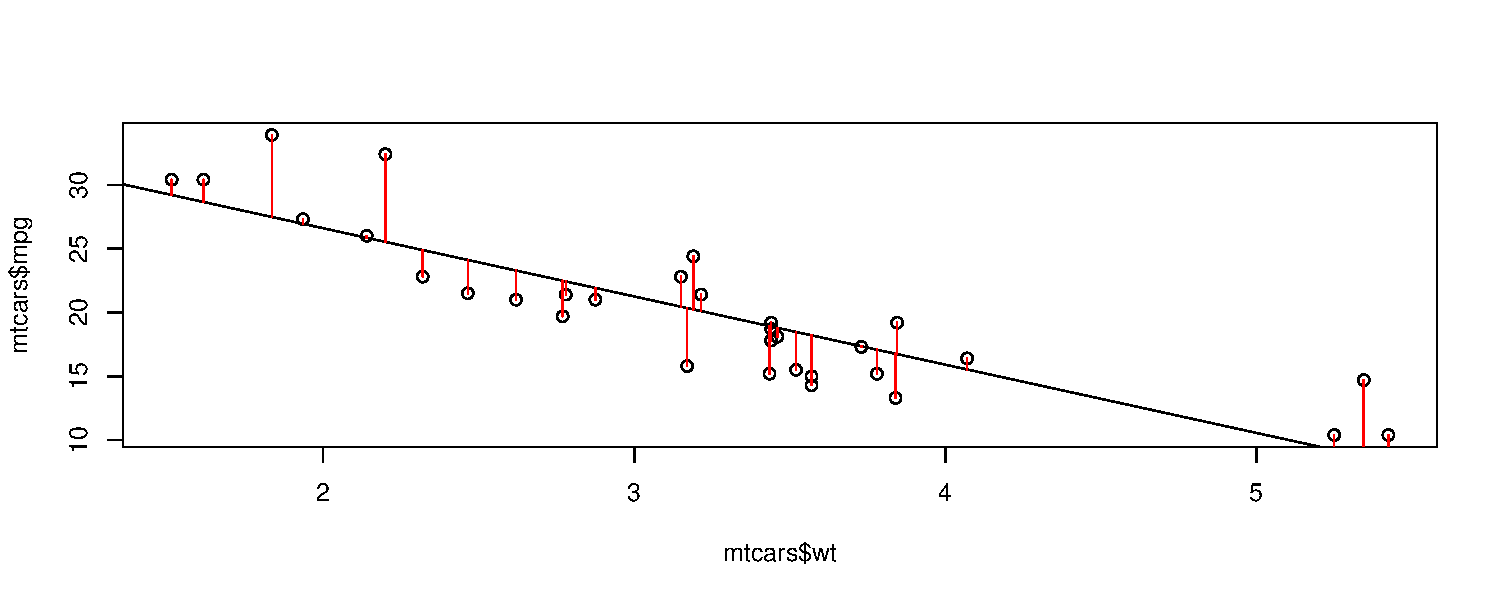
\includegraphics{LineareRegression_files/figure-beamer/unnamed-chunk-28-1.pdf}

\end{frame}

\begin{frame}[fragile]{Residuenplot}
\protect\hypertarget{residuenplot-2}{}

\begin{Shaded}
\begin{Highlighting}[]
\KeywordTok{plot}\NormalTok{(m3,}\DecValTok{2}\NormalTok{)}
\end{Highlighting}
\end{Shaded}

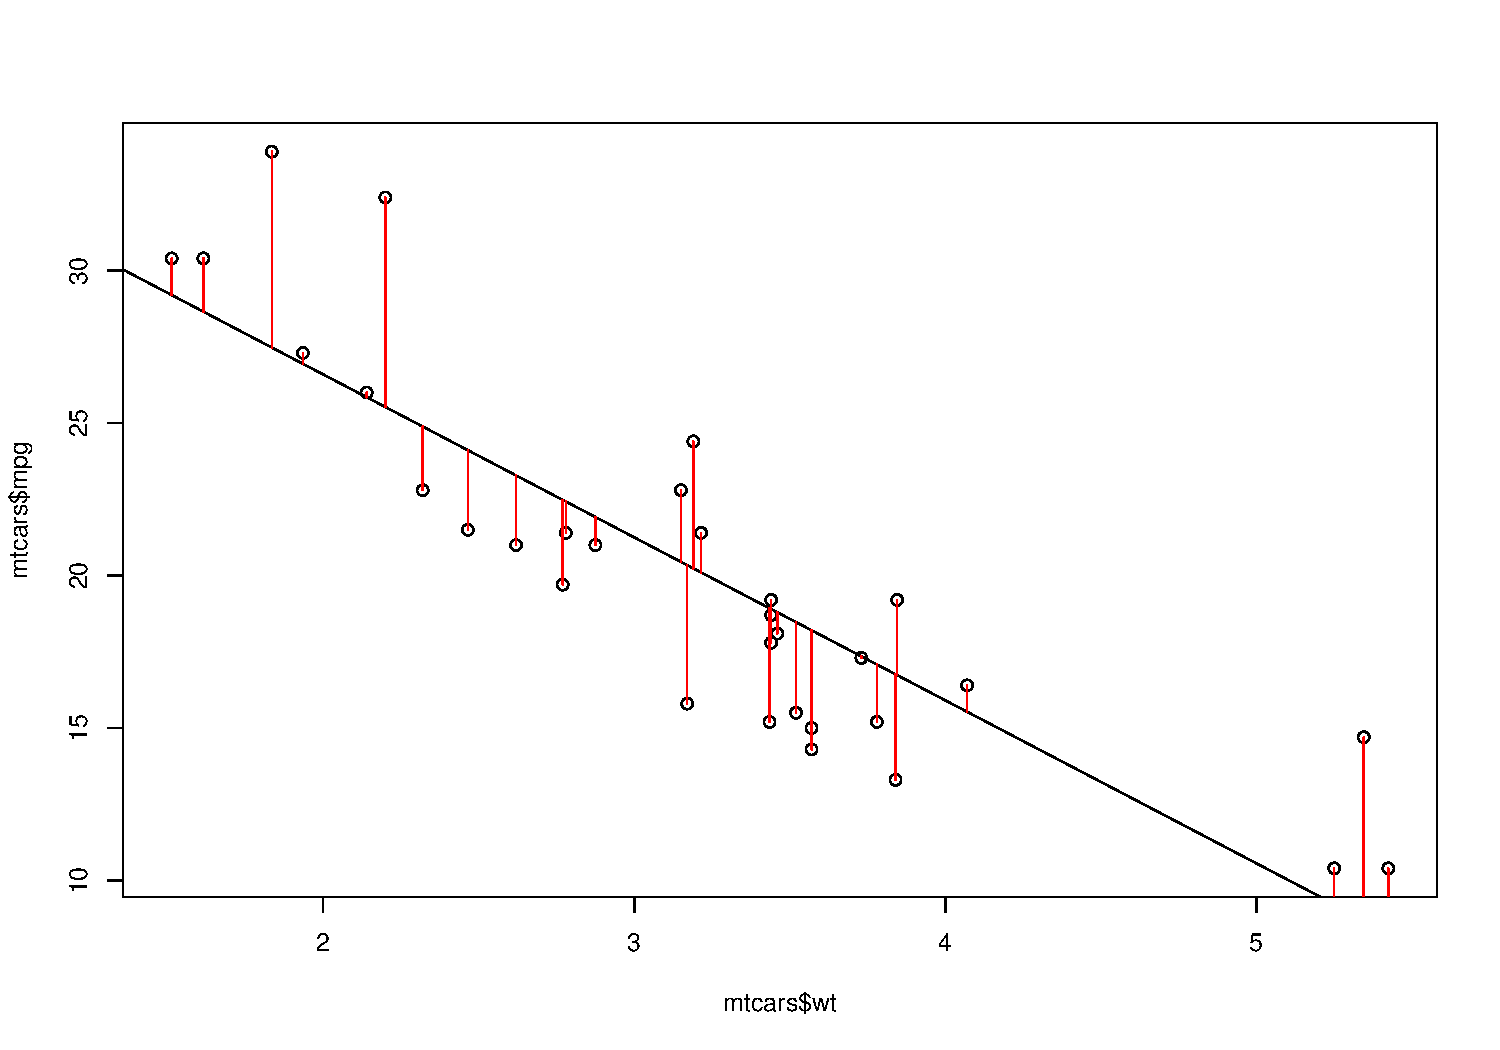
\includegraphics{LineareRegression_files/figure-beamer/unnamed-chunk-29-1.pdf}

\begin{itemize}
\tightlist
\item
  Wenn die Residuen normalverteilt sind, dann sollten sie auf der
  gleichen Linie liegen.
\end{itemize}

\end{frame}

\begin{frame}[fragile]{Regressionsdiagnostik mit Basis-R}
\protect\hypertarget{regressionsdiagnostik-mit-basis-r}{}

\begin{Shaded}
\begin{Highlighting}[]
\KeywordTok{plot}\NormalTok{(mtcars}\OperatorTok{$}\NormalTok{wt,mtcars}\OperatorTok{$}\NormalTok{mpg)}
\KeywordTok{abline}\NormalTok{(m1)}
\KeywordTok{segments}\NormalTok{(mtcars}\OperatorTok{$}\NormalTok{wt, mtcars}\OperatorTok{$}\NormalTok{mpg, mtcars}\OperatorTok{$}\NormalTok{wt, pre, }\DataTypeTok{col=}\StringTok{"red"}\NormalTok{)}
\end{Highlighting}
\end{Shaded}

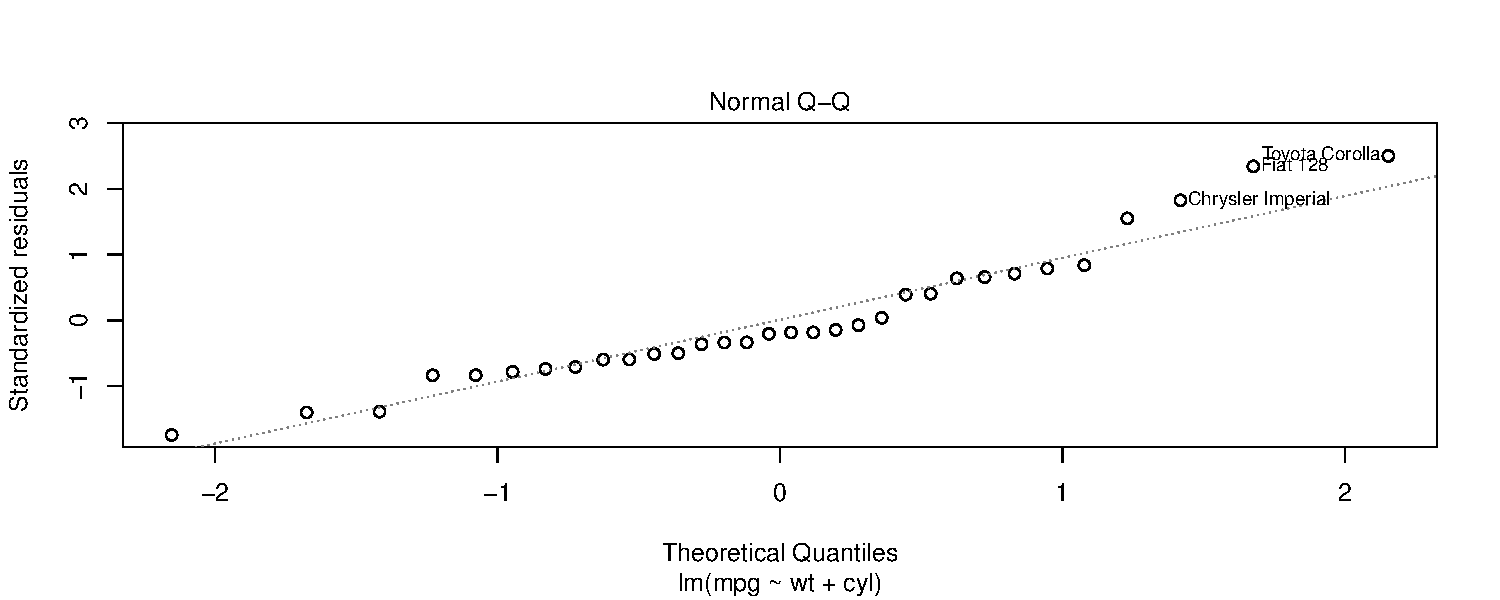
\includegraphics{LineareRegression_files/figure-beamer/unnamed-chunk-30-1.pdf}

\end{frame}

\begin{frame}[fragile]{Das \texttt{visreg}-Paket}
\protect\hypertarget{das-visreg-paket}{}

\begin{Shaded}
\begin{Highlighting}[]
\KeywordTok{install.packages}\NormalTok{(}\StringTok{"visreg"}\NormalTok{)}
\end{Highlighting}
\end{Shaded}

\begin{Shaded}
\begin{Highlighting}[]
\KeywordTok{library}\NormalTok{(visreg)}
\end{Highlighting}
\end{Shaded}

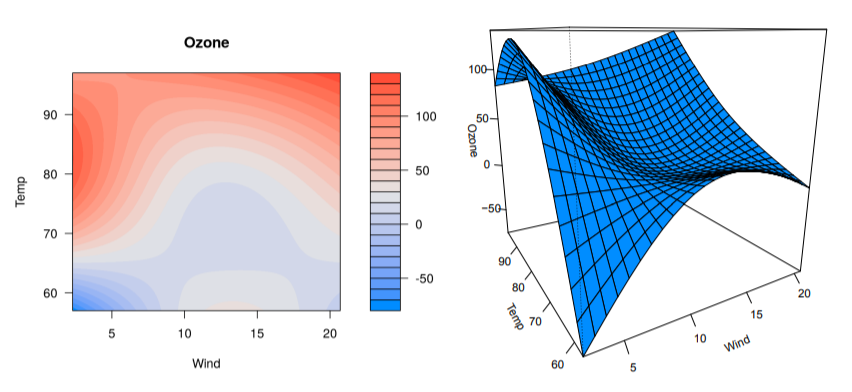
\includegraphics{figure/visreg.PNG}

\end{frame}

\begin{frame}[fragile]{Das \texttt{visreg}-Paket}
\protect\hypertarget{das-visreg-paket-1}{}

\begin{itemize}
\tightlist
\item
  Das Default-Argument für \texttt{type} ist \texttt{conditional}.
\item
  Scatterplot von \texttt{mpg} und \texttt{wt} mit Regressionslinie und
  Konfidenzbändern
\end{itemize}

\begin{Shaded}
\begin{Highlighting}[]
\KeywordTok{visreg}\NormalTok{(m1, }\StringTok{"wt"}\NormalTok{, }\DataTypeTok{type =} \StringTok{"conditional"}\NormalTok{)}
\end{Highlighting}
\end{Shaded}

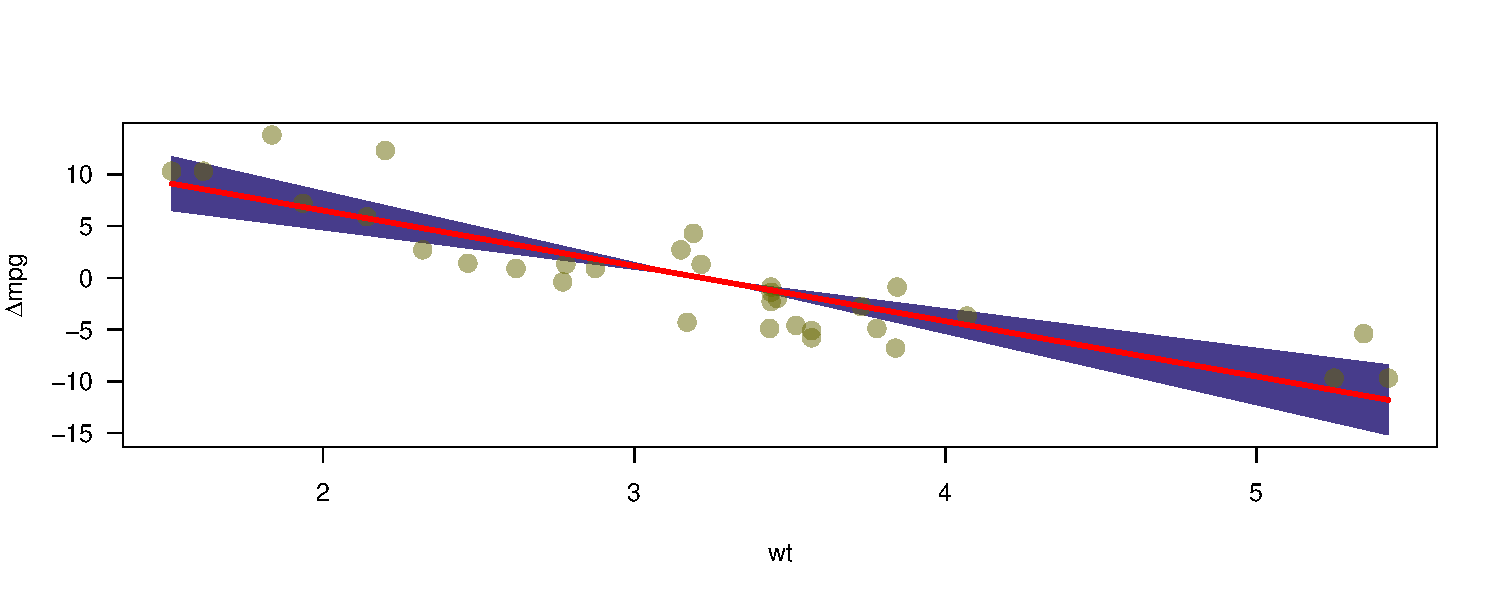
\includegraphics{LineareRegression_files/figure-beamer/unnamed-chunk-35-1.pdf}

\end{frame}

\begin{frame}[fragile]{\href{http://myweb.uiowa.edu/pbreheny/publications/visreg.pdf}{\textbf{Visualisierung
mit \texttt{visreg}}}}
\protect\hypertarget{visualisierung-mit-visreg}{}

\begin{itemize}
\tightlist
\item
  \href{http://pbreheny.github.io/visreg}{Zweites Argument} -
  Spezifikation der Kovariaten in der Graphik
\item
  Das Diagramm zeigt die Auswirkung auf den erwarteten Wert des
  Regressors, wenn die Variable x von einem Referenzpunkt auf der
  x-Achse wegbewegt wird (bei numerischen Variablen der Mittelwert).
\end{itemize}

\begin{Shaded}
\begin{Highlighting}[]
\KeywordTok{visreg}\NormalTok{(m1, }\StringTok{"wt"}\NormalTok{, }\DataTypeTok{type =} \StringTok{"contrast"}\NormalTok{)}
\end{Highlighting}
\end{Shaded}

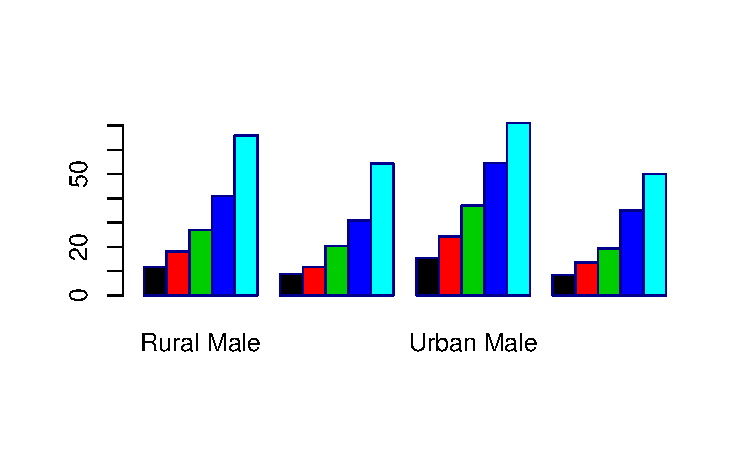
\includegraphics{LineareRegression_files/figure-beamer/unnamed-chunk-37-1.pdf}

\end{frame}

\begin{frame}[fragile]{Regression mit Faktoren}
\protect\hypertarget{regression-mit-faktoren}{}

\begin{itemize}
\tightlist
\item
  Die Effekte von Faktoren können auch mit \texttt{visreg} visualisiert
  werden:
\end{itemize}

\begin{Shaded}
\begin{Highlighting}[]
\NormalTok{mtcars}\OperatorTok{$}\NormalTok{cyl <-}\StringTok{ }\KeywordTok{as.factor}\NormalTok{(mtcars}\OperatorTok{$}\NormalTok{cyl)}
\NormalTok{m4 <-}\StringTok{ }\KeywordTok{lm}\NormalTok{(mpg }\OperatorTok{~}\StringTok{ }\NormalTok{cyl }\OperatorTok{+}\StringTok{ }\NormalTok{wt, }\DataTypeTok{data =}\NormalTok{ mtcars)}
\CommentTok{# summary(m4)}
\end{Highlighting}
\end{Shaded}

\begin{verbatim}
##              Estimate Std. Error   t value     Pr(>|t|)
## (Intercept) 33.990794  1.8877934 18.005569 6.257246e-17
## cyl6        -4.255582  1.3860728 -3.070244 4.717834e-03
## cyl8        -6.070860  1.6522878 -3.674214 9.991893e-04
## wt          -3.205613  0.7538957 -4.252065 2.130435e-04
\end{verbatim}

\end{frame}

\begin{frame}[fragile]{Effekte von Faktoren}
\protect\hypertarget{effekte-von-faktoren}{}

\begin{Shaded}
\begin{Highlighting}[]
\KeywordTok{par}\NormalTok{(}\DataTypeTok{mfrow=}\KeywordTok{c}\NormalTok{(}\DecValTok{1}\NormalTok{,}\DecValTok{2}\NormalTok{))}
\KeywordTok{visreg}\NormalTok{(m4, }\StringTok{"cyl"}\NormalTok{, }\DataTypeTok{type =} \StringTok{"contrast"}\NormalTok{)}
\KeywordTok{visreg}\NormalTok{(m4, }\StringTok{"cyl"}\NormalTok{, }\DataTypeTok{type =} \StringTok{"conditional"}\NormalTok{)}
\end{Highlighting}
\end{Shaded}

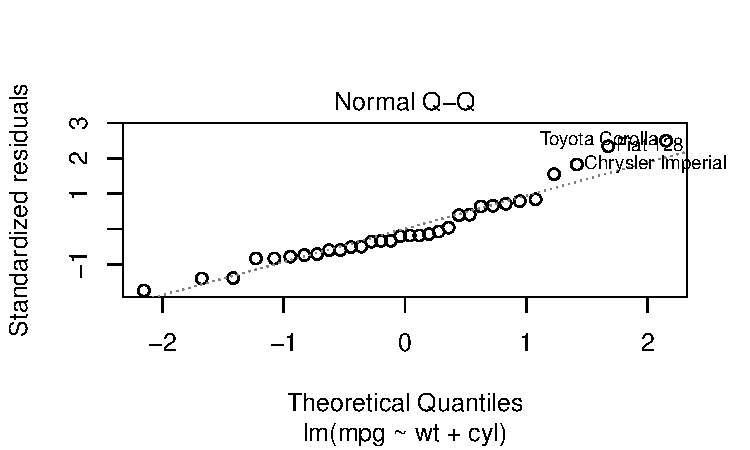
\includegraphics{LineareRegression_files/figure-beamer/unnamed-chunk-41-1.pdf}

\end{frame}

\begin{frame}[fragile]{Das Paket \texttt{visreg} - Interaktionen}
\protect\hypertarget{das-paket-visreg---interaktionen}{}

\begin{Shaded}
\begin{Highlighting}[]
\NormalTok{m5 <-}\StringTok{ }\KeywordTok{lm}\NormalTok{(mpg }\OperatorTok{~}\StringTok{ }\NormalTok{cyl}\OperatorTok{*}\NormalTok{wt, }\DataTypeTok{data =}\NormalTok{ mtcars)}
\CommentTok{# summary(m5)}
\end{Highlighting}
\end{Shaded}

\begin{verbatim}
##               Estimate Std. Error    t value     Pr(>|t|)
## (Intercept)  39.571196   3.193940 12.3894599 2.058359e-12
## cyl6        -11.162351   9.355346 -1.1931522 2.435843e-01
## cyl8        -15.703167   4.839464 -3.2448150 3.223216e-03
## wt           -5.647025   1.359498 -4.1537586 3.127578e-04
## cyl6:wt       2.866919   3.117330  0.9196716 3.661987e-01
## cyl8:wt       3.454587   1.627261  2.1229458 4.344037e-02
\end{verbatim}

\end{frame}

\begin{frame}[fragile]{Den Graphikoutput mit \texttt{layout}
kontrollieren}
\protect\hypertarget{den-graphikoutput-mit-layout-kontrollieren}{}

\begin{Shaded}
\begin{Highlighting}[]
\KeywordTok{visreg}\NormalTok{(m5, }\StringTok{"wt"}\NormalTok{, }\DataTypeTok{by =} \StringTok{"cyl"}\NormalTok{,}\DataTypeTok{layout=}\KeywordTok{c}\NormalTok{(}\DecValTok{3}\NormalTok{,}\DecValTok{1}\NormalTok{))}
\end{Highlighting}
\end{Shaded}

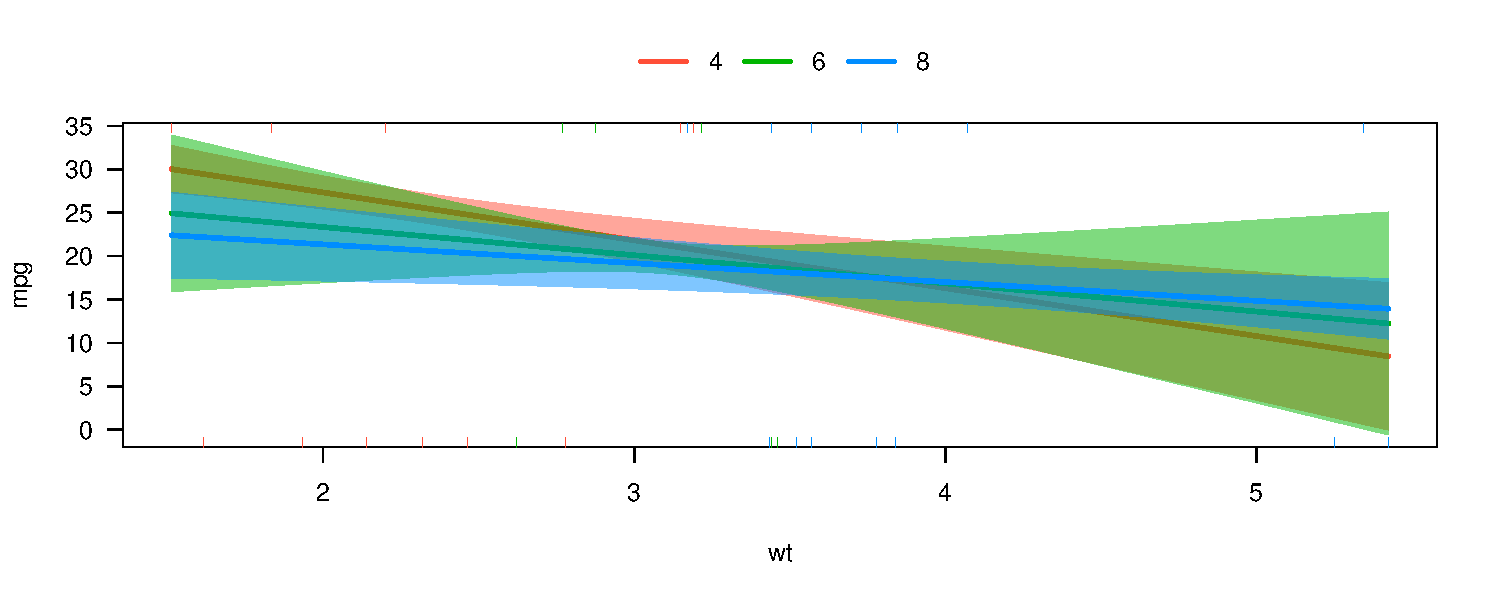
\includegraphics{LineareRegression_files/figure-beamer/unnamed-chunk-45-1.pdf}

\end{frame}

\begin{frame}[fragile]{Das Paket \texttt{visreg} - Interaktionseffekte
übereinander legen}
\protect\hypertarget{das-paket-visreg---interaktionseffekte-ubereinander-legen}{}

\begin{Shaded}
\begin{Highlighting}[]
\NormalTok{m6 <-}\StringTok{ }\KeywordTok{lm}\NormalTok{(mpg }\OperatorTok{~}\StringTok{ }\NormalTok{hp }\OperatorTok{+}\StringTok{ }\NormalTok{wt }\OperatorTok{*}\StringTok{ }\NormalTok{cyl, }\DataTypeTok{data =}\NormalTok{ mtcars)}
\end{Highlighting}
\end{Shaded}

\begin{Shaded}
\begin{Highlighting}[]
\KeywordTok{visreg}\NormalTok{(m6, }\StringTok{"wt"}\NormalTok{, }\DataTypeTok{by=}\StringTok{"cyl"}\NormalTok{, }\DataTypeTok{overlay=}\OtherTok{TRUE}\NormalTok{, }\DataTypeTok{partial=}\OtherTok{FALSE}\NormalTok{)}
\end{Highlighting}
\end{Shaded}

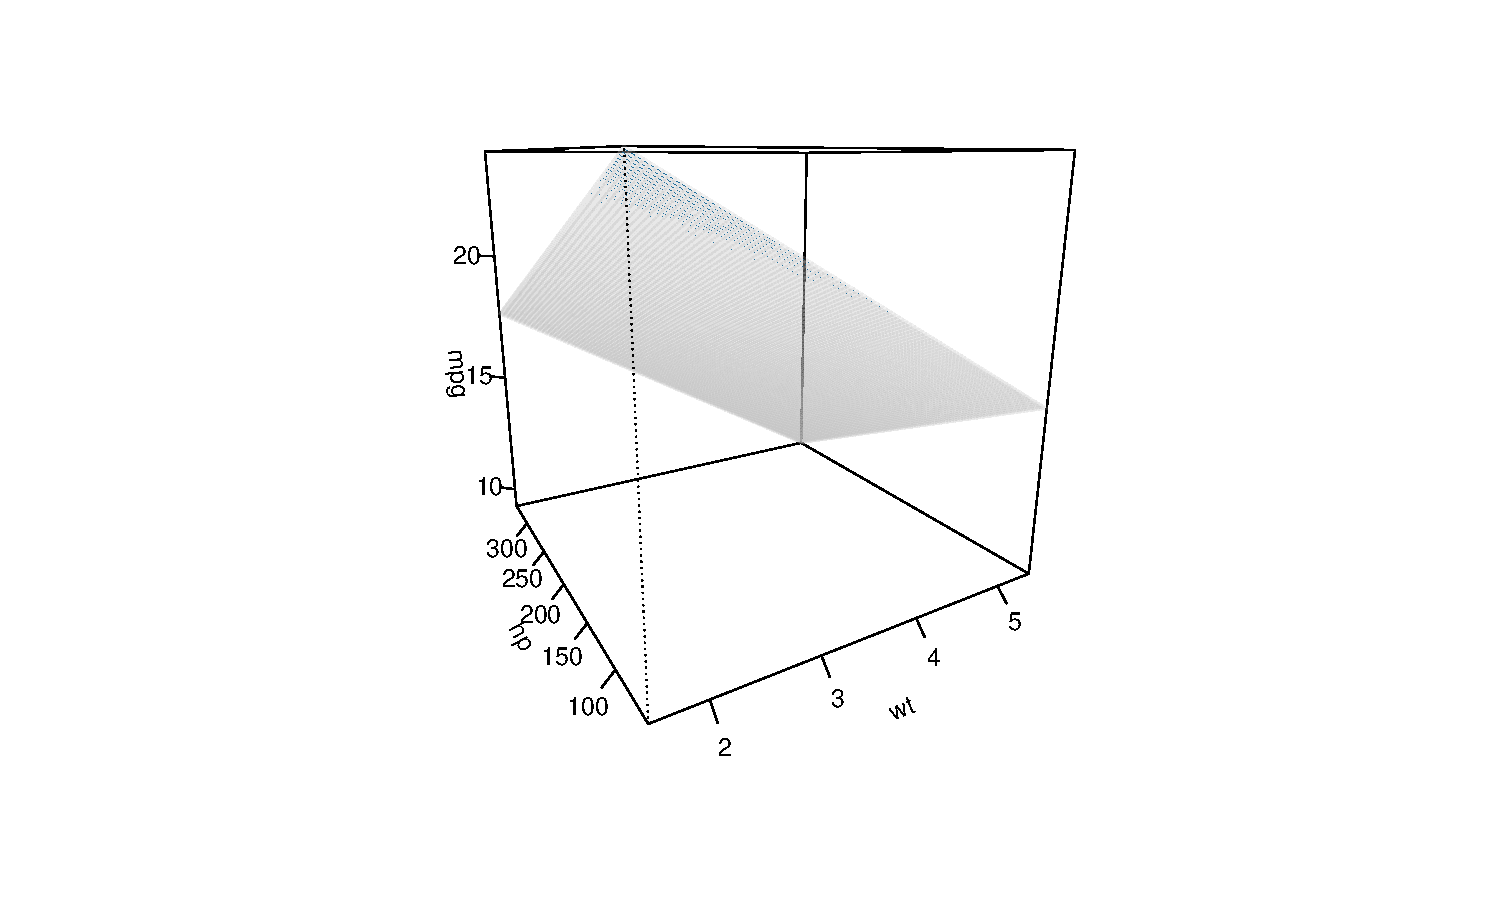
\includegraphics{LineareRegression_files/figure-beamer/unnamed-chunk-47-1.pdf}

\end{frame}

\begin{frame}[fragile]{Das Paket \texttt{visreg} - \texttt{visreg2d}}
\protect\hypertarget{das-paket-visreg---visreg2d}{}

\begin{Shaded}
\begin{Highlighting}[]
\KeywordTok{visreg2d}\NormalTok{(m6, }\StringTok{"wt"}\NormalTok{, }\StringTok{"hp"}\NormalTok{, }\DataTypeTok{plot.type =} \StringTok{"image"}\NormalTok{)}
\end{Highlighting}
\end{Shaded}

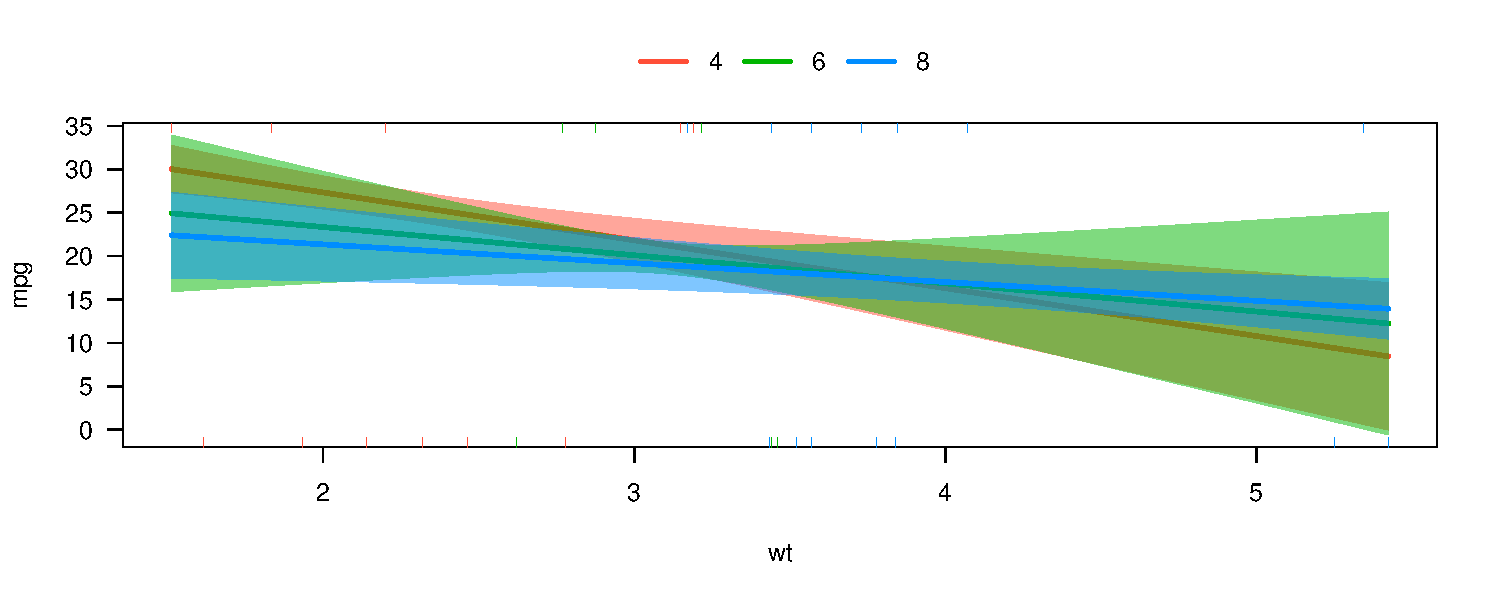
\includegraphics{LineareRegression_files/figure-beamer/unnamed-chunk-48-1.pdf}

\end{frame}

\begin{frame}[fragile]{Das Paket \texttt{visreg} - \texttt{surface}}
\protect\hypertarget{das-paket-visreg---surface}{}

\begin{Shaded}
\begin{Highlighting}[]
\KeywordTok{visreg2d}\NormalTok{(m6, }\StringTok{"wt"}\NormalTok{, }\StringTok{"hp"}\NormalTok{, }\DataTypeTok{plot.type =} \StringTok{"persp"}\NormalTok{)}
\end{Highlighting}
\end{Shaded}

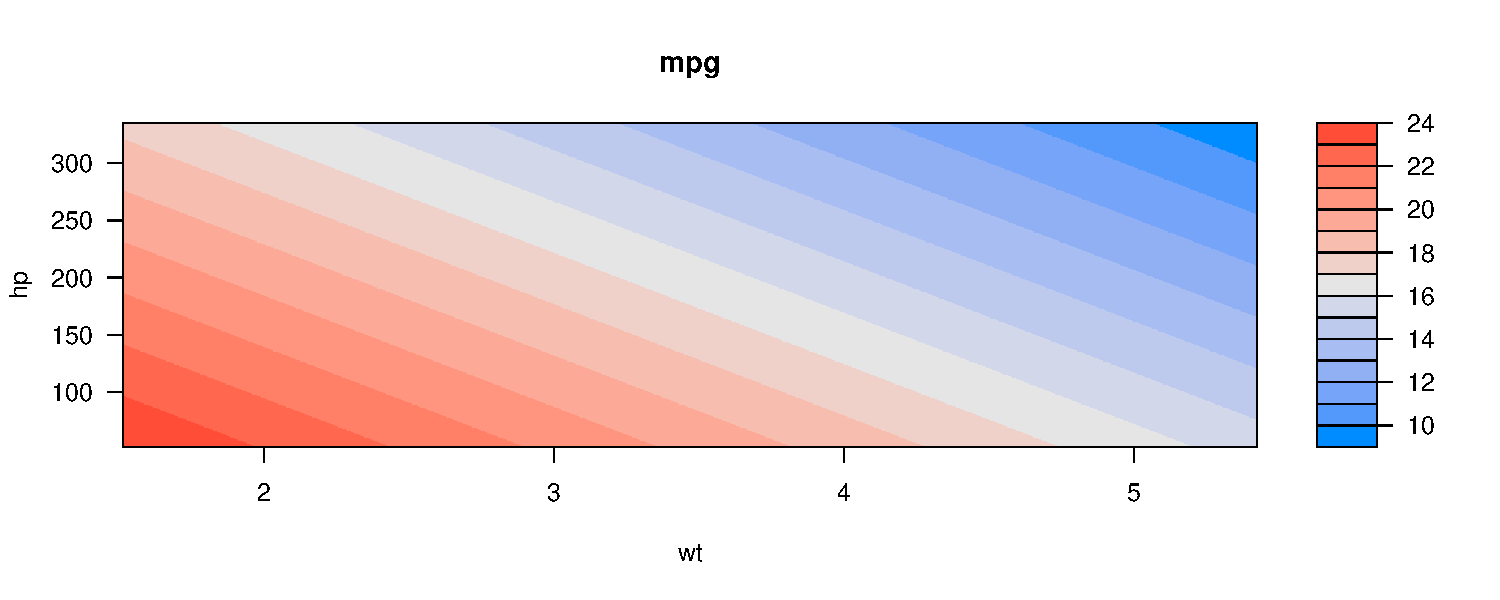
\includegraphics{LineareRegression_files/figure-beamer/unnamed-chunk-49-1.pdf}

\end{frame}

\begin{frame}[fragile]{B3A Aufgabe lineare Regression}
\protect\hypertarget{b3a-aufgabe-lineare-regression}{}

Der Datensatz \texttt{toycars} beschreibt die Route von drei
Spielzeugautos, die Rampen in verschiedenen Winkeln absteigen.

\begin{itemize}
\tightlist
\item
  angle: Rampenwinkel
\item
  distance: Entfernung die von dem Spielzeugauto zurück gelegt wird.
\item
  car: Autotyp (1, 2 or 3)
\end{itemize}

\begin{enumerate}
[a)]
\tightlist
\item
  Lese den Datensatz \texttt{toycars} ein und konvertiere die Variable
  \texttt{car} des Datensatzes in einen Faktor (\texttt{as.factor}).
\end{enumerate}

\begin{enumerate}
[(a)]
\setcounter{enumi}{1}
\tightlist
\item
  Erstelle drei Box-Plots, in denen die von den Autotypen zurückgelegte
  Strecke visualisiert wird.
\end{enumerate}

\end{frame}

\begin{frame}[fragile]{B3A Aufgabe lineare Regression II}
\protect\hypertarget{b3a-aufgabe-lineare-regression-ii}{}

\begin{enumerate}
[(a)]
\setcounter{enumi}{2}
\tightlist
\item
  Schätze für jeden Autotyp getrennt die Parameter des folgenden
  linearen Modell; nutze dafür die Funktion \texttt{lm()}
\end{enumerate}

\[ distance_i= \beta_0 + \beta_1 \cdot angle_i + \epsilon_i\]

\begin{enumerate}
[(a)]
\setcounter{enumi}{3}
\tightlist
\item
  Überprüfe die Anpassung des Modells indem Du die drei
  Regressionslinien in den Scatterplot einzeichnest (\texttt{distance}
  gegen \texttt{angle}). Spricht das \[ R^2 \] für eine gute
  Modellanpassung?
\end{enumerate}

\end{frame}

\begin{frame}[fragile]{Einen schönen Output mit dem Paket
\href{https://cran.r-project.org/web/packages/stargazer/vignettes/stargazer.pdf}{\textbf{\texttt{stargazer}}}}
\protect\hypertarget{einen-schonen-output-mit-dem-paket-stargazer}{}

erzeugen

\begin{Shaded}
\begin{Highlighting}[]
\KeywordTok{library}\NormalTok{(stargazer)}
\KeywordTok{stargazer}\NormalTok{(m3, }\DataTypeTok{type=}\StringTok{"html"}\NormalTok{)}
\end{Highlighting}
\end{Shaded}

\begin{block}{Beispiel HTML Outputs:}

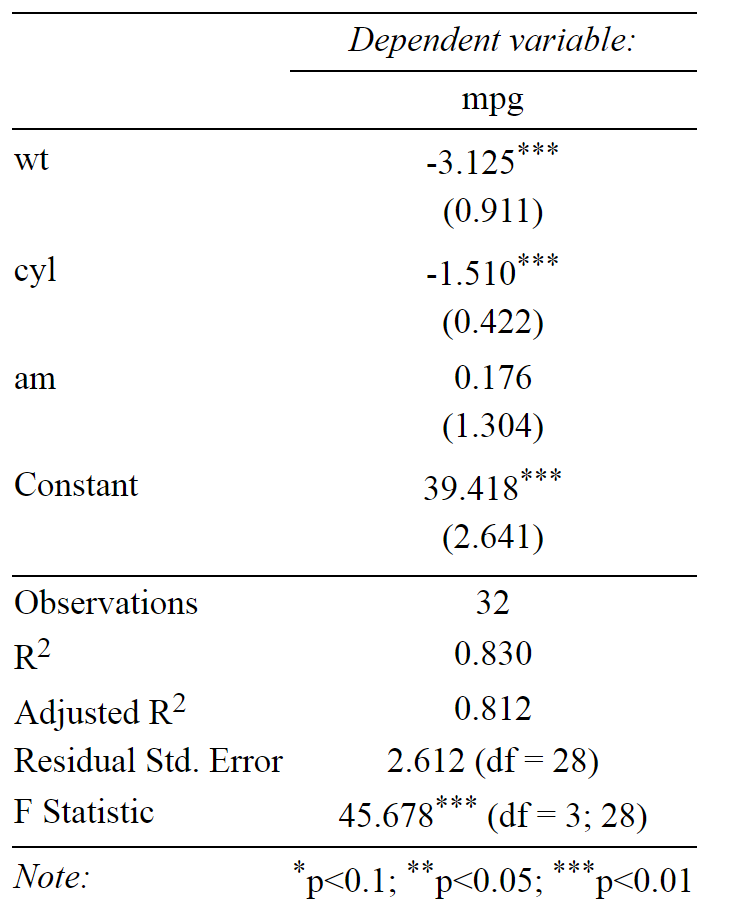
\includegraphics{figure/stargazertabex.PNG}

\end{block}

\end{frame}

\begin{frame}{Shiny App - Diagnostiken für die einfache lineare
Regression}
\protect\hypertarget{shiny-app---diagnostiken-fur-die-einfache-lineare-regression}{}

\url{https://gallery.shinyapps.io/slr_diag/}

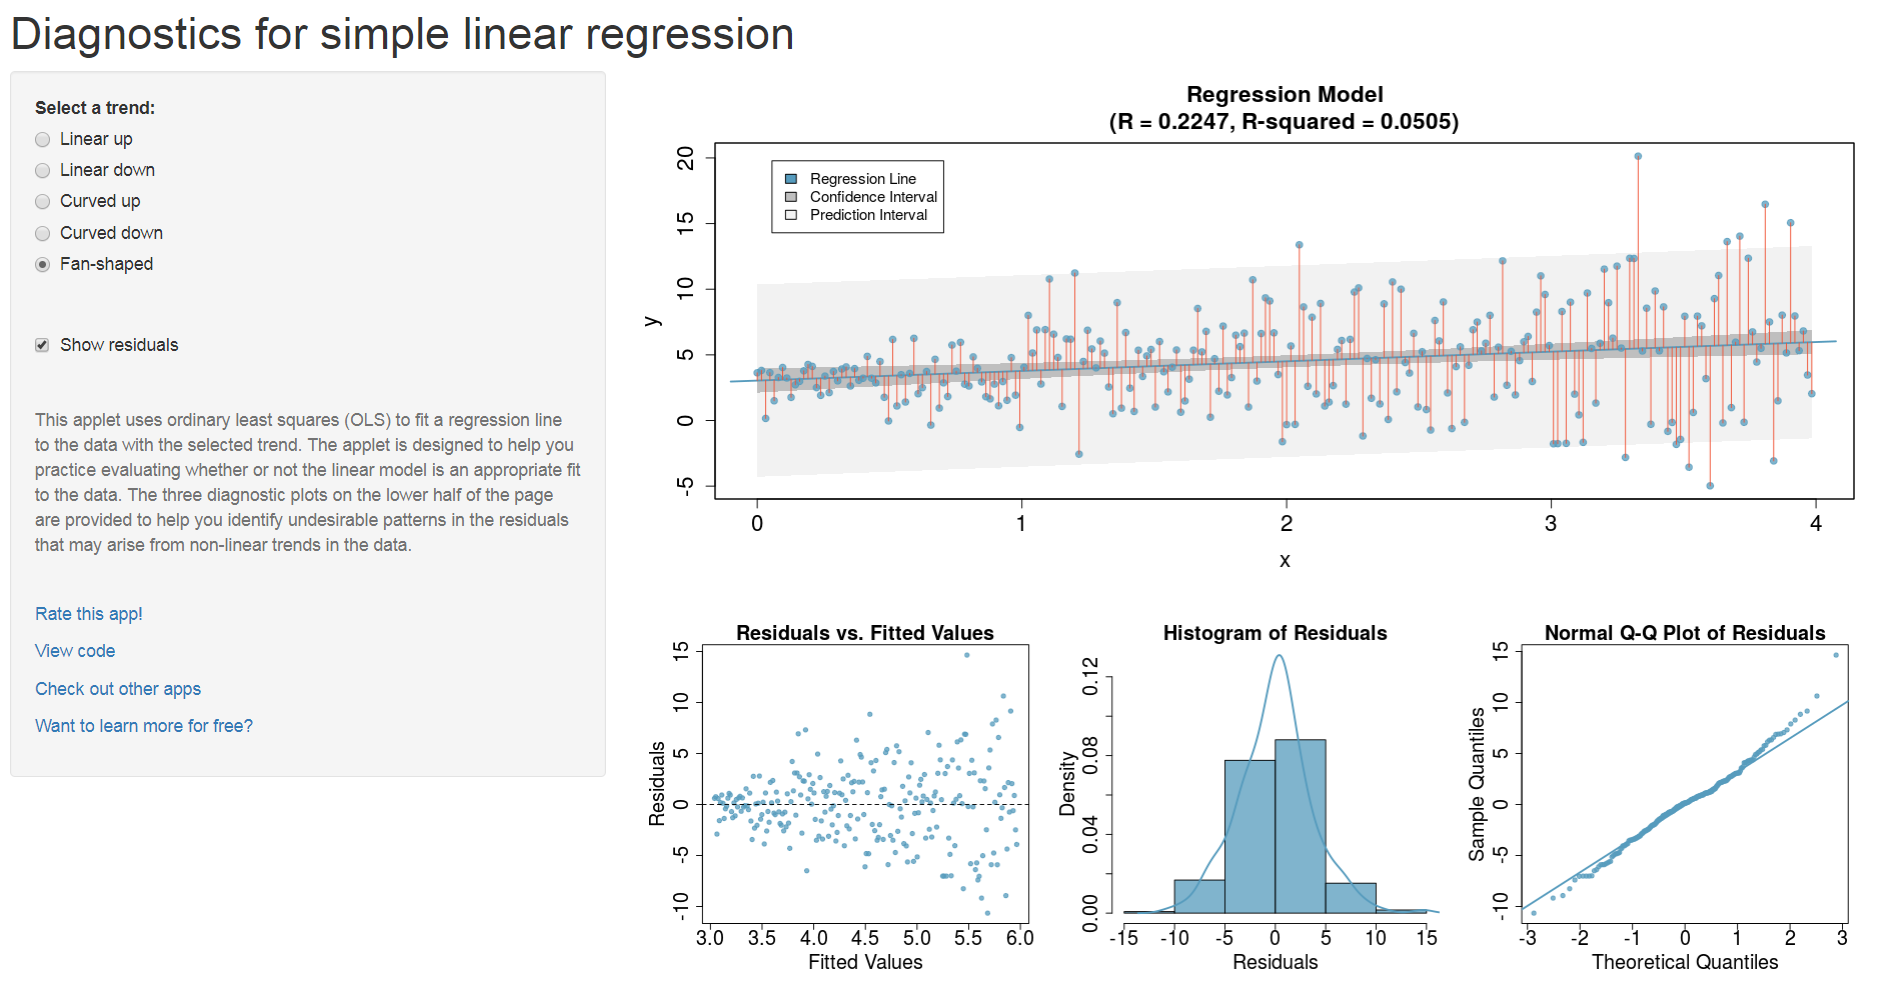
\includegraphics{figure/Diagslr.PNG}

\begin{itemize}
\item
  Shiny App -
  \href{https://gallery.shinyapps.io/simple_regression/}{\textbf{Eine
  einfache lineare Regression}}
\item
  Shiny App -
  \href{figure/https://gallery.shinyapps.io/collinearity/}{\textbf{Multikollinearität
  in multiplen Regressionen testen}}
\end{itemize}

\end{frame}

\begin{frame}[fragile]{Links - lineare Regression}
\protect\hypertarget{links---lineare-regression}{}

\begin{itemize}
\item
  Regression -
  \href{http://www.r-bloggers.com/r-tutorial-series-simple-linear-regression/}{\textbf{r-bloggers}}
\item
  Das komplette Buch von
  \href{http://cran.r-project.org/doc/contrib/Faraway-PRA.pdf}{\textbf{Faraway}}-
  sehr intuitiv geschriebenes Buch
\item
  Gute Einführung auf
  \href{http://www.statmethods.net/stats/regression.html}{\textbf{Quick-R}}
\item
  \href{https://www.r-bloggers.com/multiple-regression-part-1/}{\textbf{Multiple
  Regression}}
\item
  \href{https://www.r-bloggers.com/15-types-of-regression-you-should-know/}{\textbf{15
  Arten von Regressionen die man kennen sollte}}
\item
  \href{https://strengejacke.github.io/ggeffects/}{\textbf{\texttt{ggeffects}
  - Erzeuge saubere Datensätze mit marginellen Effekten für `ggplot' aus
  Modell Outputs}}
\end{itemize}

\end{frame}

\end{document}
